\documentclass{ctexart}

\usepackage{geometry}
\geometry{a4paper, top=2.54cm, bottom=2.54cm, left=1.91cm, right=1.91cm}
\usepackage{tocloft} %模板中用了subfigure,不加此选项会产生冲突
\renewcommand{\cftsecleader}{\cftdotfill{\cftdotsep}}
\renewcommand{\contentsname}{\bfseries 目录}% 设置”目录“左对齐(xiao xing)

\usepackage[colorlinks, linkcolor = red]{hyperref}
\usepackage{enumitem}%  列表环境
\usepackage{tcolorbox}
\tcbuselibrary{skins}
\usepackage{colortbl}
\def\mydollar{{\fontspec{Consolas}\$\ }}% 单个字体设置
\definecolor{structure}{RGB}{0,120,2}
\definecolor{main}{RGB}{0,166,82}
\definecolor{second}{RGB}{230,90,7}
\definecolor{white}{RGB}{255,255,255}

\newtcolorbox{mybox}[2][]{
    colframe = main,  
    colback = main!5,
    colbacktitle = main,
    coltitle = white, 
    title={#2},
    fonttitle=\bfseries,
    #1
}

\title{Arch Linux 学习笔记}
\author{ZiTai}
\date{\zhdate{2023/7/9}}

\begin{document}
\maketitle

\clearpage
\tableofcontents

\clearpage
\section{起步}
    学习编程相关知识,Linux 是一个不错的平台,
    它相比于 Windows 来说,它一开始就提供了很多实用的工具,
    例如 VIM 编辑器,GCC 编译工具,强大的 Shell 支持等等。
    因此,在这里记录我的 Linux 学习旅程,和大家一起分享。

    Linux 是完全开源的,从概念上讲,“Linux” 仅仅指的是一个操作系统内核,
    一个完整的操作系统还应该包括其他支持,有很多厂商使用它作为内核,然后加一些其他东西,
    例如图形化界面等等,我选择的发行版为 Arch Linux。

    在学习的过程中,我们要充分利用好现有的资源才能少走弯路。
    下面列举一些 Arch Linux 的学习资源:

    \begin{itemize}[labelindent=\parindent, leftmargin=*, align=left]
        \item 官网:\href{https://www.archlinuxcn.org/}{https://www.archlinuxcn.org/}
        \item ArchWiki:\href{https://wiki.archlinux.org/}{https://wiki.archlinux.org/}
        \item 论坛:\href{https://bbs.archlinux.org/}{https://bbs.archlinux.org/}
        \item Telegram:\href{https://t.me/archlinuxcn\_group}{https://t.me/archlinuxcn\_group}
        \item 菜鸟教程:\href{https://www.runoob.com/linux/linux-tutorial.html}{https://www.runoob.com/linux/linux-tutorial.html}
    \end{itemize}


    Linux 上还有一个工具帮助我们学习各种指令,使用 man 帮助手册,可以查询命令的使用。
    例如,在 Linux 命令行里运行 \texttt{man man} 命令,可以查询命令 \texttt{man} 的用法。

\section{Linux 的目录组织方式}
    在命令行中输入:

\begin{mybox}{}
    \texttt{cd /}% 输入反斜线 \:\textbackslash
    
    \texttt{ls}
\end{mybox}

    就可以列出 Linux 系统目录结构的全貌。
    根据发行版的不同,大致类似于这样:

    \begin{figure}[htbp]
        \centering
        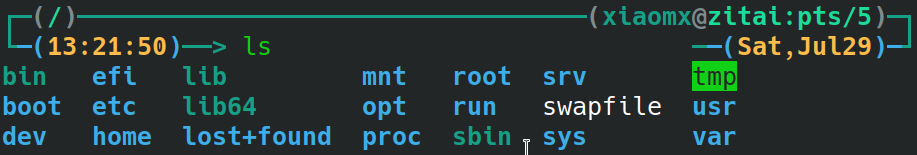
\includegraphics[width=0.80\textwidth]{images/directory/1.png}
        %\caption{}
    \end{figure}

    树状目录结构:

    \begin{figure}[htbp]
        \centering
        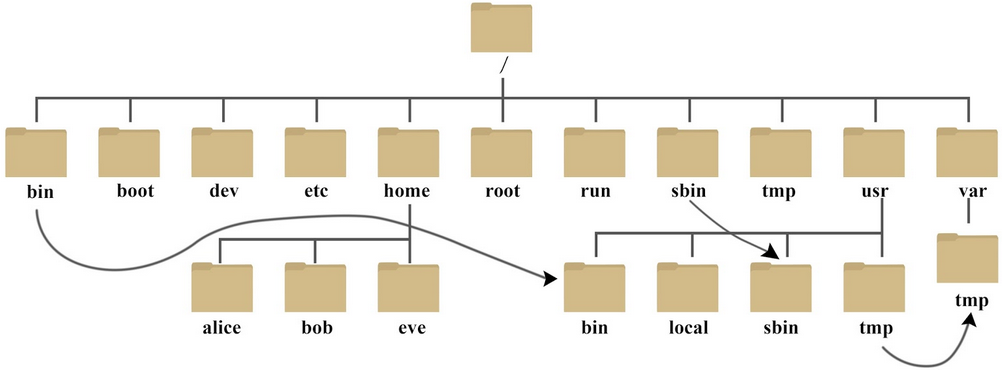
\includegraphics[width=0.80\textwidth]{images/directory/2.png}
        \caption{Linux 树状目录结构\ {}图片来自于菜鸟教程}
    \end{figure}

    /bin:
    bin 是 Binaries(二进制文件)的缩写,用于存放最经常使用的命令。
    例如,检查当前路径的命令 \texttt{pwd} 就存放在这里。

    /boot:
    这里存放的是启动 Linux 时使用的一些核心文件,包括一些连接文件以及镜像文件。

    /dev:
    dev 是 Device(设备) 的缩写,该目录下存放的是 Linux 的外部设备,
    在 Linux 中访问设备的方式和访问文件的方式是相同的(Linux 号称一切对象皆文件)。

    /etc:
    etc 是 Etcetera(等等) 的缩写,这个目录用来存放所有系统管理所需要的配置文件和子目录。
    这些配置文件主要用于设置和管理系统的各种参数、服务和应用程序的行为。
    常见的 /etc 目录下文件的作用:
    
    \begin{enumerate}[labelindent=\parindent, leftmargin=*, align=left]
        %\item /etc/passwd: 存储了系统用户的账户信息,如用户名、用户ID、用户所属组ID、用户家目录路径等。
        %\item /etc/group: 包含了用户组的信息,如组名、组ID和组成员等。
        %\item /etc/shadow: 存储了加密后的用户密码信息。
        %\item /etc/hosts: 用于配置主机名与IP地址的映射关系,可以手动指定主机名的解析。
        \item /etc/resolv.conf: 配置系统的DNS解析服务器,用于域名解析。
        %\item /etc/network/interfaces或/etc/sysconfig/network-scripts/ifcfg-*: 用于配置网络接口的IP地址、网关、DNS等网络参数。
        %\item /etc/fstab: 定义了文件系统的挂载点及其选项,在系统启动时自动挂载。
        \item /etc/pacman.d: 这个目录下的文件是与包管理器 Pacman 相关的配置文件。
        \item /etc/ssh/sshd\_config: SSH 服务的配置文件,用于定义 SSH 服务器的行为和安全选项。
    \end{enumerate}

    /home:
    用户的主目录,在 Linux 中,每个用户都有一个自己的目录,
    一般该目录名是以用户的账号命名的,如上图中的 alice、bob 和 eve。
    这个目录下还有一个 lost+found 目录。

    /lib:
    lib 是 Library(库) 的缩写,这个目录里存放着系统最基本的动态连接共享库,
    其作用类似于 Windows 里的 DLL 文件。几乎所有的应用程序都需要用到这些共享库。
    这个目录通常包含 32 位系统库文件。
    在过去,许多 Linux 系统都是 32 位的,因此系统库文件被放置在 /lib 目录中。
    即使现在许多系统已经迁移到 64 位架构,但为了向后兼容性,仍然保留了这个目录。
    对于 64 位系统而言,/lib 目录中的链接指向了 /usr/lib 目录。
    lib64 目录:这个目录通常包含 64 位系统库文件。
    随着 64 位架构的普及,许多 Linux 系统都从 32 位切换到了 64 位。
    为了与 32 位库文件进行区分,并且为了纯粹的 64 位系统能够正常工作,引入了/lib64 目录。
    在 64 位系统中,/lib64 目录中的链接指向了 /usr/lib 目录。

    /lost+found:
    这个目录一般情况下是空的,当系统非法关机后,这里就存放了一些文件。
    /home 目录下的 lost+found 和根目录 /下的lost+found 目录没有本质上的区别,
    都是用于存放与该用户相关的丢失文件的恢复数据。
    当文件系统发生错误或损坏时,一些数据可能会被系统放置到该目录中。
    管理员可以检查并恢复这些丢失的文件。

    /media:
    linux 系统会自动识别一些设备,例如 U 盘、光驱等等,当识别后,Linux 会把识别的设备挂载到这个目录下。

    /mnt:
    系统提供该目录是为了让用户临时挂载别的文件系统的,
    我们可以将光驱挂载在 /mnt/ 上,然后进入该目录就可以查看光驱里的内容了。

    /opt:
    opt 是 optional(可选) 的缩写,通常用于存放第三方应用程序(optional software)的安装目录。
    比如你安装一个 ORACLE 数据库则就可以放到这个目录下。默认是空的。
    它有以下用途和优点:

    \begin{itemize}[labelindent=\parindent, leftmargin=*, align=left]
        \item 存放第三方应用程序:
                /opt目录下可以存放与操作系统本身无关的第三方软件,
                这些软件通常不会与操作系统的其他部分混合在一起。
                这样做有助于保持系统的整洁,并且容易删除或更新这些应用程序。
        \item 独立安装位置:
                相比将第三方应用程序安装在系统默认的路径下(如/usr/bin、/usr/local/bin等),
                将其安装到 /opt 目录下可以将其与系统自带的软件分开。
                这样做有助于防止操作系统和应用程序之间的冲突,并且便于对应用程序进行独立管理。
        \item 统一的目录结构:
                /opt 目录提供了一个统一的目录结构,
                使得用户和管理员可以更轻松地找到和访问已安装的第三方应用程序。
                这种结构通常包括以应用程序名称命名的子目录,
                每个子目录下包含了与该应用程序相关的二进制文件、库文件、配置文件等。
    \end{itemize}

    需要注意的是,/opt 目录并不是所有第三方应用程序的默认安装目录。
    有些应用程序可能会选择不同的位置进行安装,因此在安装新的软件时,
    记得参考其官方文档或安装说明来确定正确的目录。

    /proc:
    proc 是 Processes(进程) 的缩写,/proc 是一种伪文件系统(也即虚拟文件系统),
    存储的是当前内核运行状态的一系列特殊文件,这个目录是一个虚拟的目录,它是系统内存的映射,
    我们可以通过直接访问这个目录来获取系统信息。
    这个目录的内容不在硬盘上而是在内存里,我们也可以直接修改里面的某些文件,
    比如可以通过下面的命令来屏蔽主机的 \texttt{ping} 命令,使别人无法 \texttt{ping} 你的机器:

    \begin{mybox}
        \texttt{echo 1 > /proc/sys/net/ipv4/icmp\_echo\_ignore\_all}
    \end{mybox}

    /root:
    该目录为系统管理员,也称作超级权限者的用户主目录。
    一般用户没有权限进入。

    /sbin:
    s 就是 Super User 的意思,是 Superuser Binaries (超级用户的二进制文件) 的缩写,这里存放的是系统管理员使用的系统管理程序。

    % /selinux:
    % 这个目录是 Redhat/CentOS 所特有的目录,Selinux 是一个安全机制,类似于 windows 的防火墙,但是这套机制比较复杂,这个目录就是存放selinux相关的文件的。

    /srv:
    该目录存放一些服务启动之后需要提取的数据。

    /sys:
    这是 Linux2.6 内核的一个很大的变化。
    该目录下安装了 2.6 内核中新出现的一个文件系统 sysfs 。
    sysfs 文件系统集成了下面 3 种文件系统的信息:
    针对进程信息的 proc 文件系统、针对设备的 devfs 文件系统以及针对伪终端的 devpts 文件系统。
    该文件系统是内核设备树的一个直观反映。
    当一个内核对象被创建的时候,对应的文件和目录也在内核对象子系统中被创建。

    /tmp:
    tmp 是 temporary(临时) 的缩写这个目录是用来存放一些临时文件的。
    它是一个设置了"sticky"权限的目录,也称为sticky directory。
    "sticky"权限是一种特殊的权限,它对于多用户环境下的临时文件夹具有一定的作用。
    当一个目录具有 sticky 权限时,
    只有目录的所有者、文件的所有者和超级用户才能删除或重命名该目录下的文件。
    其他普通用户无法删除或改变不属于自己的文件。
    /tmp 目录被用作存放临时文件的地方,这些文件通常由各个程序或用户生成,但并不需要长时间保留。
    设置 /tmp 目录为 sticky 权限可以确保在多个用户共享同一目录时,
    每个用户只能删除或修改自己创建的文件,从而增加了数据的安全性和隐私保护。
    将 /tmp 目录设置为 sticky 权限还能减少对磁盘空间的滥用。
    由于该目录下的文件往往是临时性的,sticky 权限可以阻止用户意外或恶意地删除其他用户的文件,从而减少了磁盘空间的浪费。

    /usr:
    usr 是 unix shared resources(共享资源) 的缩写,这是一个非常重要的目录,
    用户的很多应用程序和文件都放在这个目录下,类似于 windows 下的 program files 目录。

    /usr/bin:
    系统用户使用的应用程序。

    /usr/sbin:
    超级用户使用的比较高级的管理程序和系统守护程序。

    /usr/src:
    内核源代码默认的放置目录。

    /var:
    var 是 variable(变量) 的缩写,
    这个目录中存放着在不断扩充着的东西,我们习惯将那些经常被修改的目录放在这个目录下。包括各种日志文件。

    /run:
    是一个临时文件系统,存储系统启动以来的信息。
    当系统重启时,这个目录下的文件应该被删掉或清除。
    如果你的系统上有 /var/run 目录,应该让它指向 run。


\clearpage
\section{pacman 包管理器}
    % /etc/pacman.d/mirrorlist: 这个文件列出了可用的软件源镜像列表。通过选择合适的镜像,可以提高软件包下载速度。

    % /etc/pacman.d/gnupg: 该目录包含了Pacman使用的GPG密钥环。这些密钥用于验证软件包的身份和完整性。

    % /etc/pacman.d/hooks/: 该目录包含了Pacman操作期间要运行的钩子脚本。这些脚本可以在安装、升级或删除软件包时执行自定义操作。

    % /etc/pacman.d/makepkg.conf: 这个文件是用于构建和打包软件包的配置文件。你可以在其中定义一些选项,如编译器标志、构建工具和依赖等。

    % /etc/pacman.d/*.conf: 除了上述文件之外,/etc/pacman.d目录还包含其他的配置文件,用于定义Pacman的行为和选项。这些文件的名称以.conf结尾,并且提供了各种配置选项。

\clearpage
\section{SSH}
    % /etc/ssh/ssh\_config 和 /etc/ssh/sshd\_config 是 SSH 协议相关的配置文件,它们在功能和使用上有以下区别:

    % /etc/ssh/ssh\_config: 这个文件是SSH客户端(即远程连接其他主机时使用的客户端)的配置文件。它用于设置SSH客户端的默认行为和选项。在该文件中,可以配置客户端的参数,如连接超时时间、身份验证方法、密钥算法、端口等。该文件作用于客户端,影响的是你从本地计算机连接到远程主机的行为。

    % /etc/ssh/sshd\_config: 这个文件是SSH服务器(即接受远程连接的主机)的配置文件。它用于设置SSH服务器的默认行为和选项。在该文件中,可以配置服务器的参数,如监听的端口、允许的用户、身份验证方式、访问限制等。该文件作用于服务器端,影响的是其他计算机通过SSH连接到你的计算机时的行为。

\clearpage
\section{常用 Bash 命令}
\begin{mybox}{文件管理}
    \texttt{cat}

    \texttt{file}

    \texttt{find}

    \texttt{less}

    \texttt{locate}

    \texttt{more}

    \texttt{mv}

    \texttt{rm}

    \texttt{touch}

    \texttt{which}

    \texttt{cp}

    \texttt{whereis}

    \texttt{read}
\end{mybox}

\begin{mybox}{文档编辑}
    \texttt{fold}

    \texttt{grep}
\end{mybox}

\begin{mybox}{磁盘管理}
    \texttt{cd}

    \texttt{df}

    \texttt{mkdir}

    \texttt{pwd}

    \texttt{stat}

    \texttt{tree}

    \texttt{ls}
\end{mybox}

\begin{mybox}{系统管理}
    \texttt{date}

    \texttt{exit}

    \texttt{sleep}

    \texttt{halt}
    
    \texttt{kill}

    \texttt{login}

    \texttt{logname}

    \texttt{logout}

    \texttt{top}

    \texttt{reboot}

    \texttt{shutdown}
    
    \texttt{sudo}

    \texttt{chsh}

    \texttt{who}

    \texttt{whoami}

    \texttt{whois}
\end{mybox}

\begin{mybox}{系统设置}
    \texttt{clear}

    \texttt{alias}

    \texttt{unalias}

    \texttt{dircolors}

    \texttt{bind}

    \texttt{clock}

    \texttt{export}

    \texttt{passwd}

    \texttt{time}
\end{mybox}

\begin{mybox}{备份压缩}
    \texttt{gunzip}

    \texttt{dump}
    
    \texttt{gzip}

    \texttt{restore}

    \texttt{tar}
    
    \texttt{unzip}

    \texttt{zip}

    \texttt{zipinfo}
\end{mybox}


\begin{mybox}{设备管理}
    \texttt{poweroff}
\end{mybox}

\clearpage
\section{ArchLinux 常见操作}



% \begin{mybox}{\href{https://www.runoob.com/linux/linux-comm-cat.html}{cat}}
%     用于连接文件并打印到标准输出设备上
%     \tcbline
%     \texttt{cat [-AbeEnstTuv] [--help] [--version] filename}
%     \tcbline
%     参数说明:

%     \begin{itemize}
%       \item -n 或 --number:由 1 开始对所有输出的行数编号。
%       \item -b 或 --number-nonblank:和 -n 相似,只不过对于空白行不编号。
%       \item -s 或 --squeeze-blank:当遇到有连续两行以上的空白行,就代换为一行的空白行。
%       \item -v 或 --show-nonprinting:使用 \^ 和 M- 符号,除了 LFD 和 TAB 之外。
%       \item -E 或 --show-ends : 在每行结束处显示 \$。
%       \item -T 或 --show-tabs: 将 TAB 字符显示为 \^I。
%       \item -A, --show-all:等价于 -vET。
%       \item -e:等价于"-vE"选项;
%       \item -t:等价于"-vT"选项;
%     \end{itemize}
% \end{mybox}

% \begin{mybox}{\href{https://www.runoob.com/linux/linux-comm-chmod.html}{chmod}}
%     控制用户对文件的权限的命令
%     \tcbline
%     \texttt{chmod [-cfvR] [--help] [--version] mode file...}
% \end{mybox}

% \begin{mybox}{\href{https://www.runoob.com/linux/linux-comm-file.html}{file}}
%     用于辨识文件类型
%     \tcbline
%     \texttt{file [-bcLvz][-f <名称文件>][-m <魔法数字文件>...][文件或目录...]}
%     \tcbline
%     参数说明:

%     \begin{itemize}
%       \item -b 列出辨识结果时,不显示文件名称。
%       \item -c 详细显示指令执行过程,便于排错或分析程序执行的情形。
%       \item -f<名称文件> 指定名称文件,其内容有一个或多个文件名称时,让 file 依序辨识这些文件,格式为每列一个文件名称。
%       \item -L 直接显示符号连接所指向的文件的类别。
%       \item -m<魔法数字文件> 指定魔法数字文件。
%       \item -v 显示版本信息。
%       \item -z 尝试去解读压缩文件的内容。
%       \item [文件或目录...] 要确定类型的文件列表,多个文件之间使用空格分开,可以使用 shell 通配符匹配多个文件。
%     \end{itemize}
% \end{mybox}

% \begin{mybox}{\href{https://www.runoob.com/linux/linux-comm-find.html}{find}}
%     \tcbline
%     \texttt{find [path] [expression]}
%     \tcbline
%     参数说明:

%     path 是要查找的目录路径,可以是一个目录或文件名,也可以是多个路径,多个路径之间用空格分隔,如果未指定路径,则默认为当前目录。

%     expression 是可选参数,用于指定查找的条件,可以是文件名、文件类型、文件大小等等。
% \end{mybox}

% \begin{mybox}{\href{https://www.runoob.com/linux/linux-comm-less.html}{less}}
%     less 与 more 类似,less 可以随意浏览文件,支持翻页和搜索,支持向上翻页和向下翻页
%     \tcbline
%     \texttt{less [参数] 文件 }
%     \tcbline
%     参数说明:

%     \begin{itemize}
%         \item -b <缓冲区大小> 设置缓冲区的大小
%         \item -e 当文件显示结束后,自动离开
%         \item -f 强迫打开特殊文件,例如外围设备代号、目录和二进制文件
%         \item -g 只标志最后搜索的关键词
%         \item -i 忽略搜索时的大小写
%         \item -m 显示类似more命令的百分比
%         \item -N 显示每行的行号
%         \item -o <文件名> 将less 输出的内容在指定文件中保存起来
%         \item -Q 不使用警告音
%         \item -s 显示连续空行为一行
%         \item -S 行过长时间将超出部分舍弃
%         \item -x <数字> 将"tab"键显示为规定的数字空格
%         \item /字符串:向下搜索"字符串"的功能
%         \item ?字符串:向上搜索"字符串"的功能
%         \item n:重复前一个搜索(与 / 或 ? 有关)
%         \item N:反向重复前一个搜索(与 / 或 ? 有关)
%         \item b 向上翻一页
%         \item d 向后翻半页
%         \item h 显示帮助界面
%         \item Q 退出less 命令
%         \item u 向前滚动半页
%         \item y 向前滚动一行
%         \item 空格键 滚动一页
%         \item 回车键 滚动一行
%         \item [pagedown]: 向下翻动一页
%         \item [pageup]: 向上翻动一页
%     \end{itemize}
% \end{mybox}
\end{document}
